\documentclass[12pt]{amsart}
\usepackage[T1]{fontenc}
\usepackage[utf8]{inputenc}

\usepackage[top=1.95cm, bottom=1.95cm, left=2.35cm, right=2.35cm]{geometry}


\usepackage{wrapfig}

\usepackage{hyperref}
\usepackage{enumitem}
\usepackage{tcolorbox}
\usepackage{float}
\usepackage{cleveref}
\usepackage{multicol}
\usepackage{fancyvrb}
\usepackage{enumitem}
\usepackage{amsmath}
\usepackage{textcomp}
\usepackage[french]{babel}
\frenchsetup{StandardItemLabels=true}
\usepackage[
    type={CC},
    modifier={by-nc-sa},
	version={4.0},
]{doclicense}

\usepackage{tnsmath}

\DeclareMathOperator{\taille}{\tau}

\newtheorem{fact}{Fait}
\newtheorem*{proof*}{Preuve}

\newtheorem{remark}{Remarque}[section]

\NewDocumentCommand{\area}{m}{\mathrm{Aire}(#1)}
\NewDocumentCommand{\perim}{m}{\mathrm{Perim}(#1)}

\setlength\parindent{0pt}


\begin{document}

\title{BROUILLON - Inégalités isopérimétriques restreintes}
\author{Christophe BAL}
\date{18 Jan. 2025 -- 19 Jan. 2025}
\maketitle


\begin{center}
	\hrule\vspace{.3em}
	{
		\fontsize{1.35em}{1em}\selectfont
		\textbf{Mentions \og légales \fg}
	}
			
	\vspace{0.45em}
	\doclicenseThis
	\hrule
\end{center}



\setcounter{tocdepth}{2}
\tableofcontents


% ------------- %


\newpage
%\section{Les rectangles}
%
%\begin{fact} \label{iso-rect}
	Considérons tous les rectangles de périmètre fixé $p$. Parmi tous ces rectangles, celui d'aire maximale est le carré de côté $c = \num{.25} p$.
\end{fact}


\begin{proof}
	Une preuve courante est d'exprimer l'aire du rectangle comme un polynôme du 2\ieme\ degré en $L$ par exemple.%
	\footnote{
		L'aire est donnée par $L \ell = L (\num{.5} p - L)$ qui est maximale en $L_M = \num{.25} p$ (moyenne des racines), d'où $\ell_M = \num{.25} p = L_M$.
	}
	On peut en fait faire plus simplement grâce au dessin suivant où les rectangles $1$, $2$ et $3$ sont isométriques au rectangle vert étudié de dimension $L \times \ell$.

	\begin{center}
		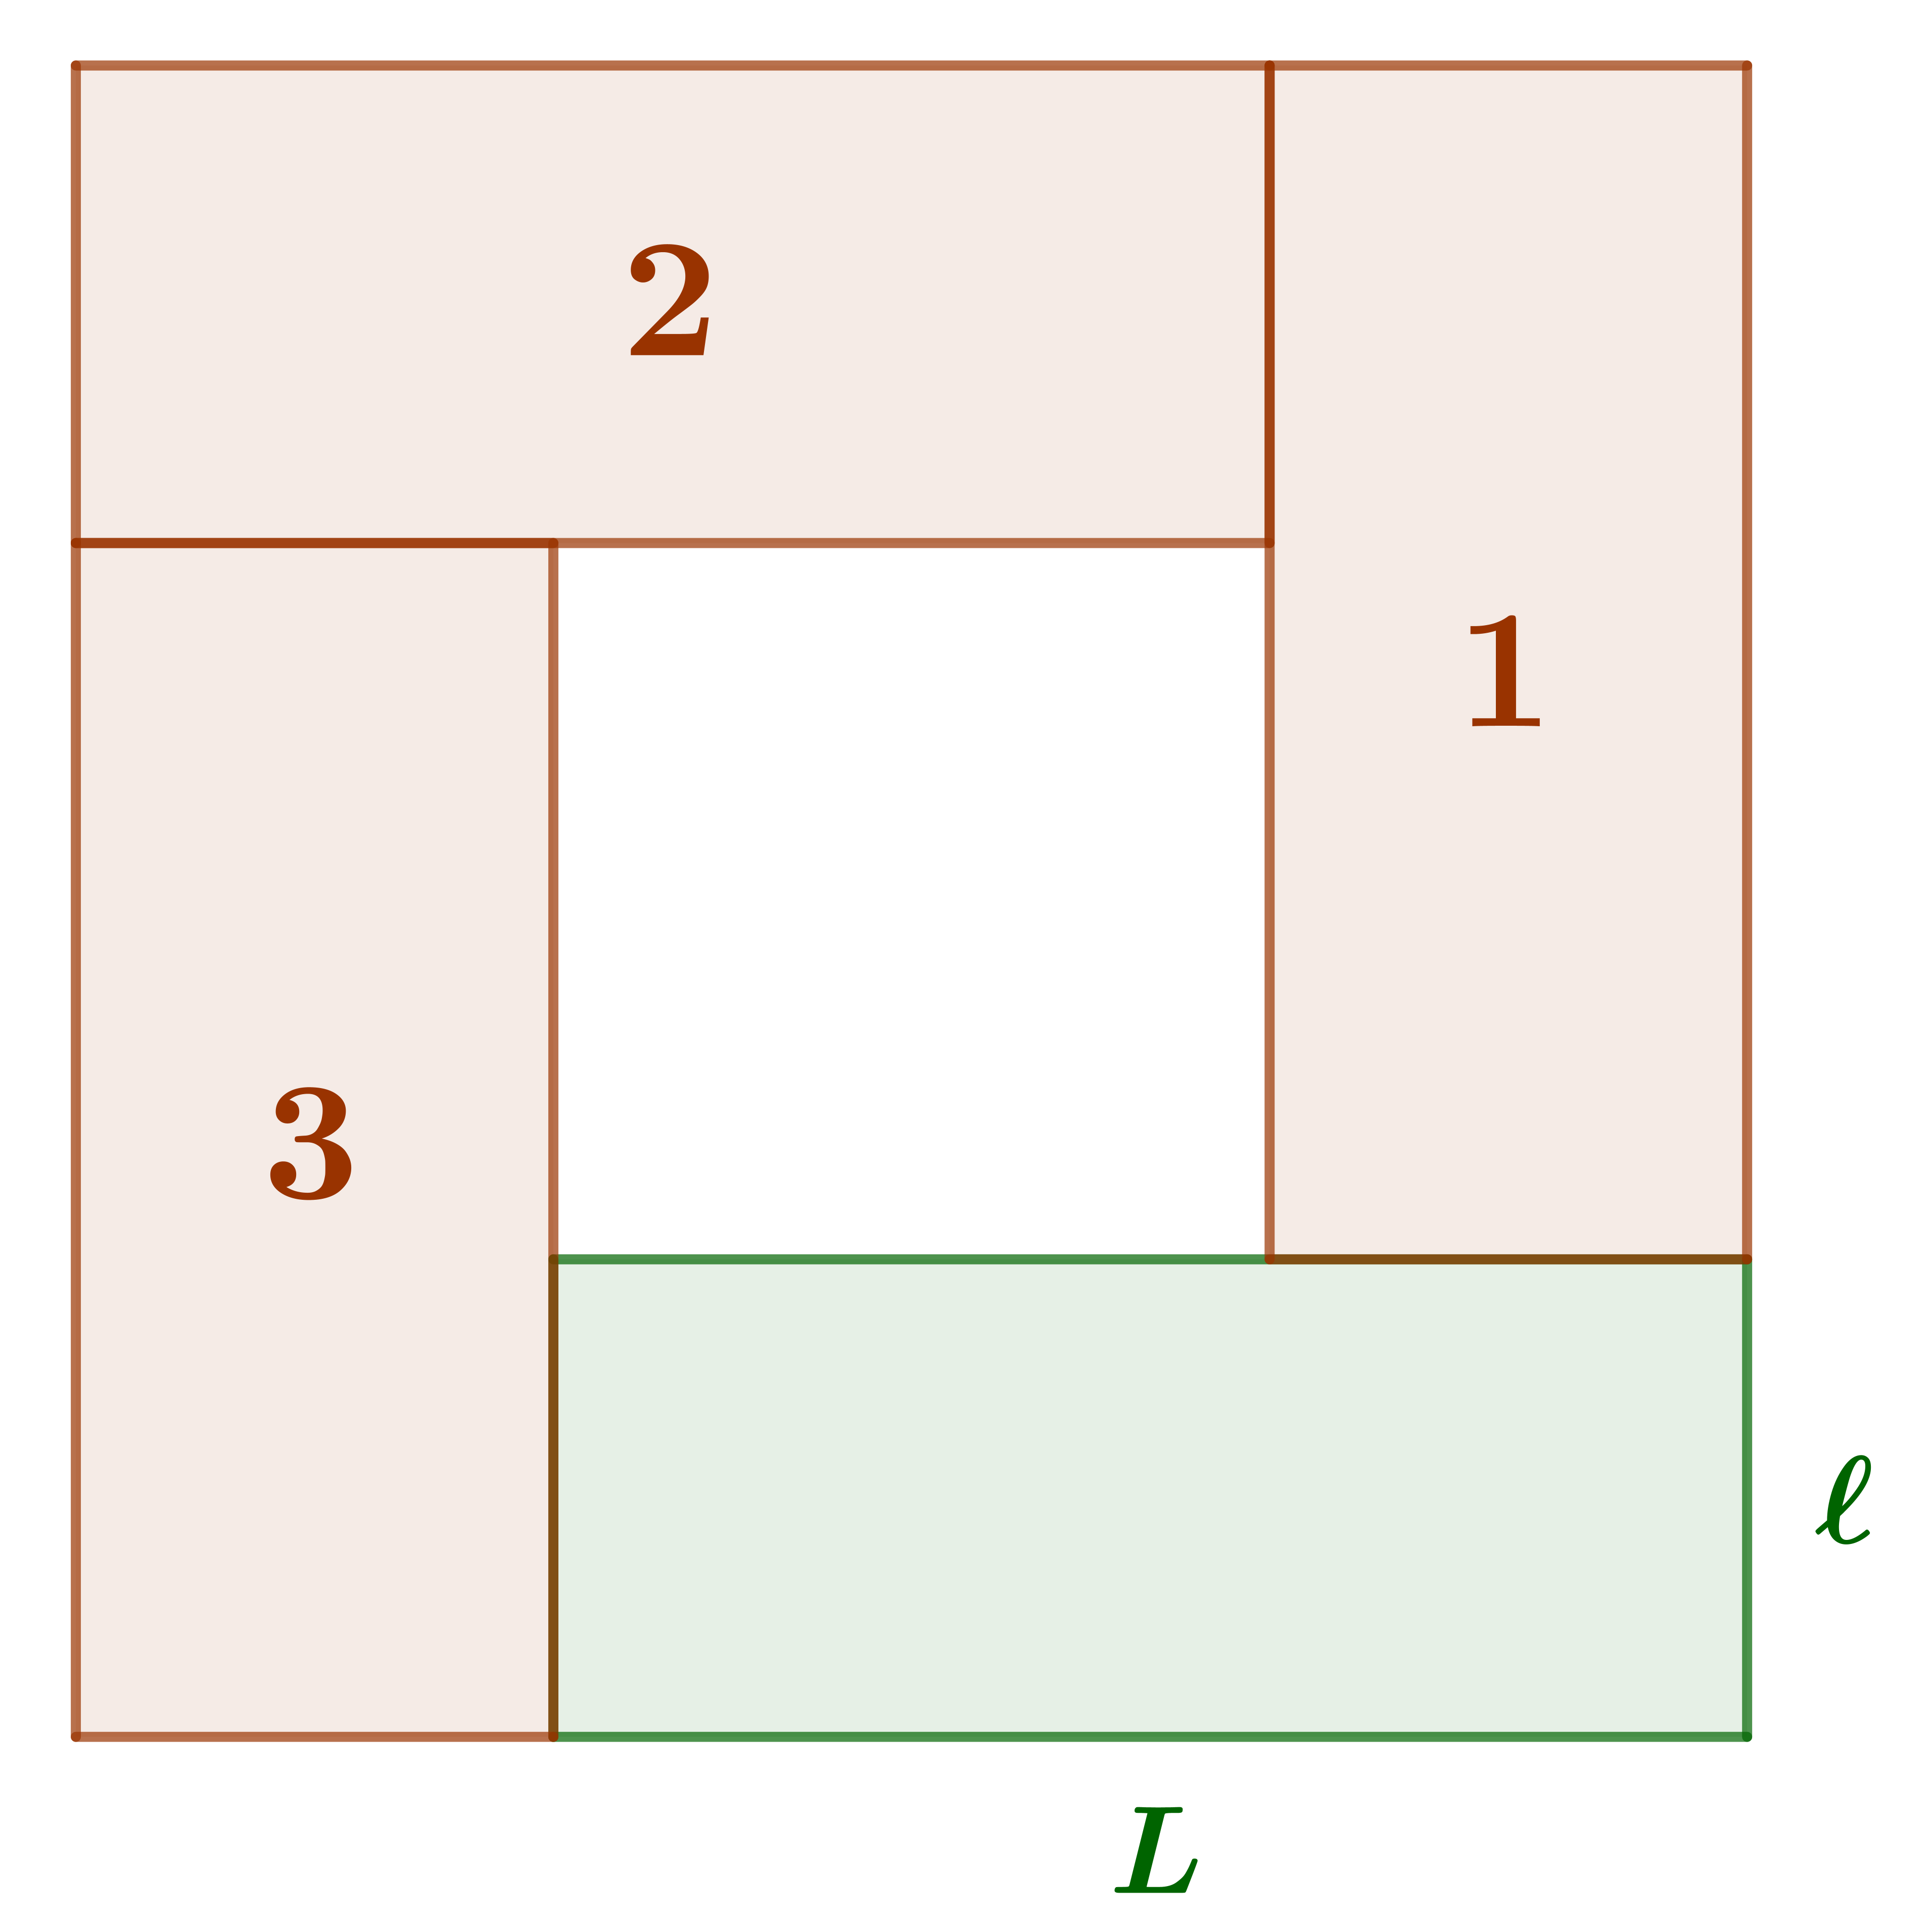
\includegraphics[scale=.4]{content/rectangle/rectangle.png}
	\end{center}
	
	Le raisonnement tient alors aux constations suivantes accessibles à un collégien.
	%
	\begin{enumerate}
		\item Le grand carré a une aire supérieure ou égale à $4 L \ell$.

		\item Le grand carré a un périmètre égal à $4 (L + \ell)$.

		\item Via une homothétie de rapport \num{.5}\,, nous obtenons un carré d'aire supérieure ou égale à $\num{.5}^2 \times 4 L \ell =  L \ell$, et de périmètre égal à $\num{.5} \times 4 (L + \ell) = 2 (L + \ell)$.
	\end{enumerate}
	
	Donc pour tout rectangle de périmètre $p = 2 (L + \ell)$ et d'aire $L \ell$, nous pouvons construire un carré de périmètre identique, mais avec une aire supérieure ou égale à  $L \ell$. Joli! Non?
\end{proof}


\begin{remark}
	Au passage, nous avons pour $(L ; \ell) \in \big( \RRsp \big)^2$, $4 L \ell \leq (L + \ell)^2$, c'est-à-dire $2 L \ell \leq L^2 + \ell^2$, d'où $\sqrt{L \ell} \leq \sqrt{\frac12 (L^2 + \ell^2)}$, soit la comparaison des moyennes géométriques et quadratiques d'ordre $2$.
\end{remark}

%
%
%% ------------- %
%
%
%\section{Les parallélogrammes}
%
%\begin{fact} \label{iso-para}
	Considérons tous les parallélogrammes de périmètre fixé $p$. Parmi tous ces parallélogrammes, un seul est d'aire maximale, c'est le carré de côté $c = \num{.25} p$.
\end{fact}


\begin{proof}
	Le calcul de l'aire d'un parallélogramme, voir le dessin ci-dessous, nous donne 
	$\area{ABCD} = \area{ABHH^{\,\prime}}$ et 
	$\perim{ABCD} \geq \perim{ABHH^{\,\prime}}$, 
	avec égalité uniquement si $ABCD$ est un rectangle. 
	
	\begin{center}
		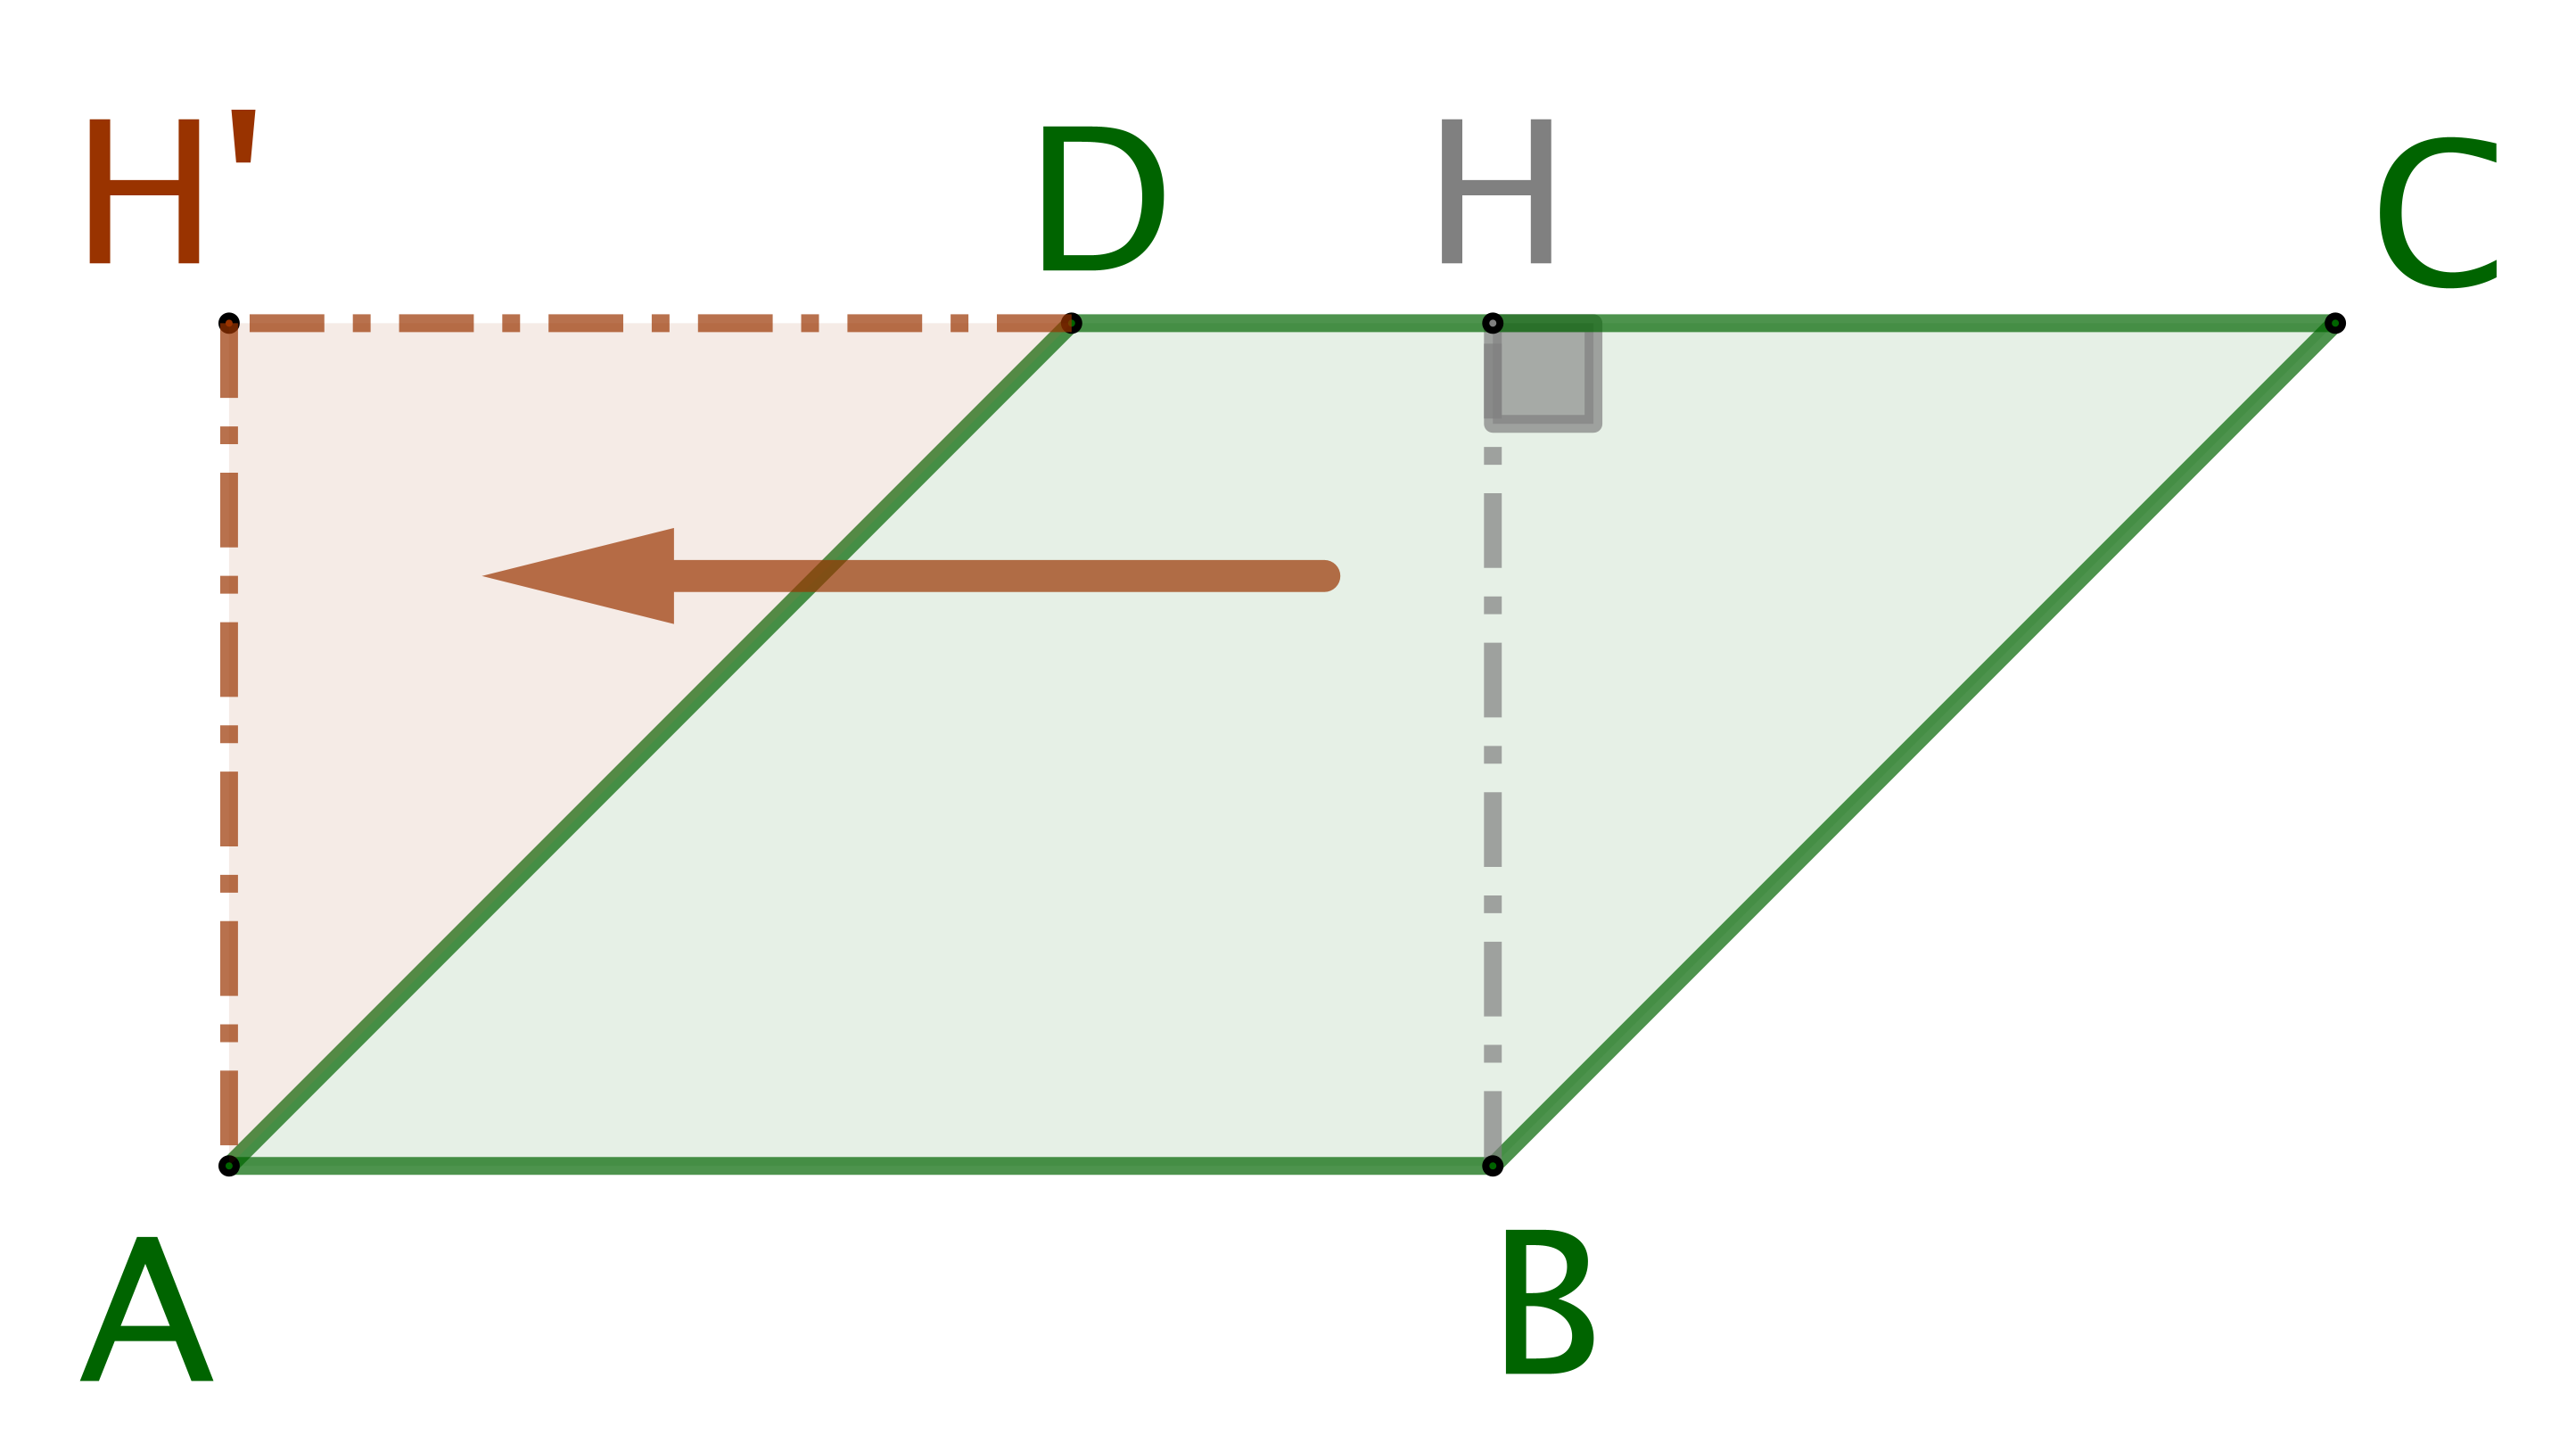
\includegraphics[scale=.4]{content/parallelogram/para-2-rect.png}
	\end{center}
	
	Via une homothétie de rapport $r = \frac{\perim{ABCD}}{\perim{ABHH^{\,\prime}}} \geq 1$, nous obtenons un rectangle 
	de périmètre égal à $p$,
	et d'aire supérieure ou égale à $\area{ABCD}$, 
	avec égalité uniquement si $ABCD$ est un rectangle.
	Nous revenons à la situation du fait \ref{iso-rect} qui permet de conclure très facilement.
\end{proof}


% ----------------------- %


\begin{remark}
	Une méthode analytique devient pénible ici, car il faut, par exemple, prendre en compte l'angle au sommet $A$ du parallélogramme. L'auteur préfère battre en retraite en clôturant cette remarque ici.
%	\footnote{
%		Et oui, l'auteur est un lâche.
%	}
\end{remark}

%
%
%% ------------- %
%
%
%\section{Les triangles avec un côté fixé}
%
%\begin{fact} \label{tri-one-side-fixed}
	Considérons tous les triangles de périmètre fixé, et ayant tous un côté en commun.
	Parmi tous ces triangles, il en existe un seul d'aire maximale, c'est le triangle isocèle ayant pour base le côté commun.
\end{fact}


\begin{proof}
	Soit $ABC$ un triangle de périmètre $p$, et fixons le côté $[AB]$. 
	Pour tout point $M$ sur la parallèle à $(AB)$ passant par $C$, nous savons que $\area{ABM} = \area{ABC}$. Notons alors $O$ le point sur cette parallèle tel que $ABO$ soit isocèle en $O$.

	\begin{center}
		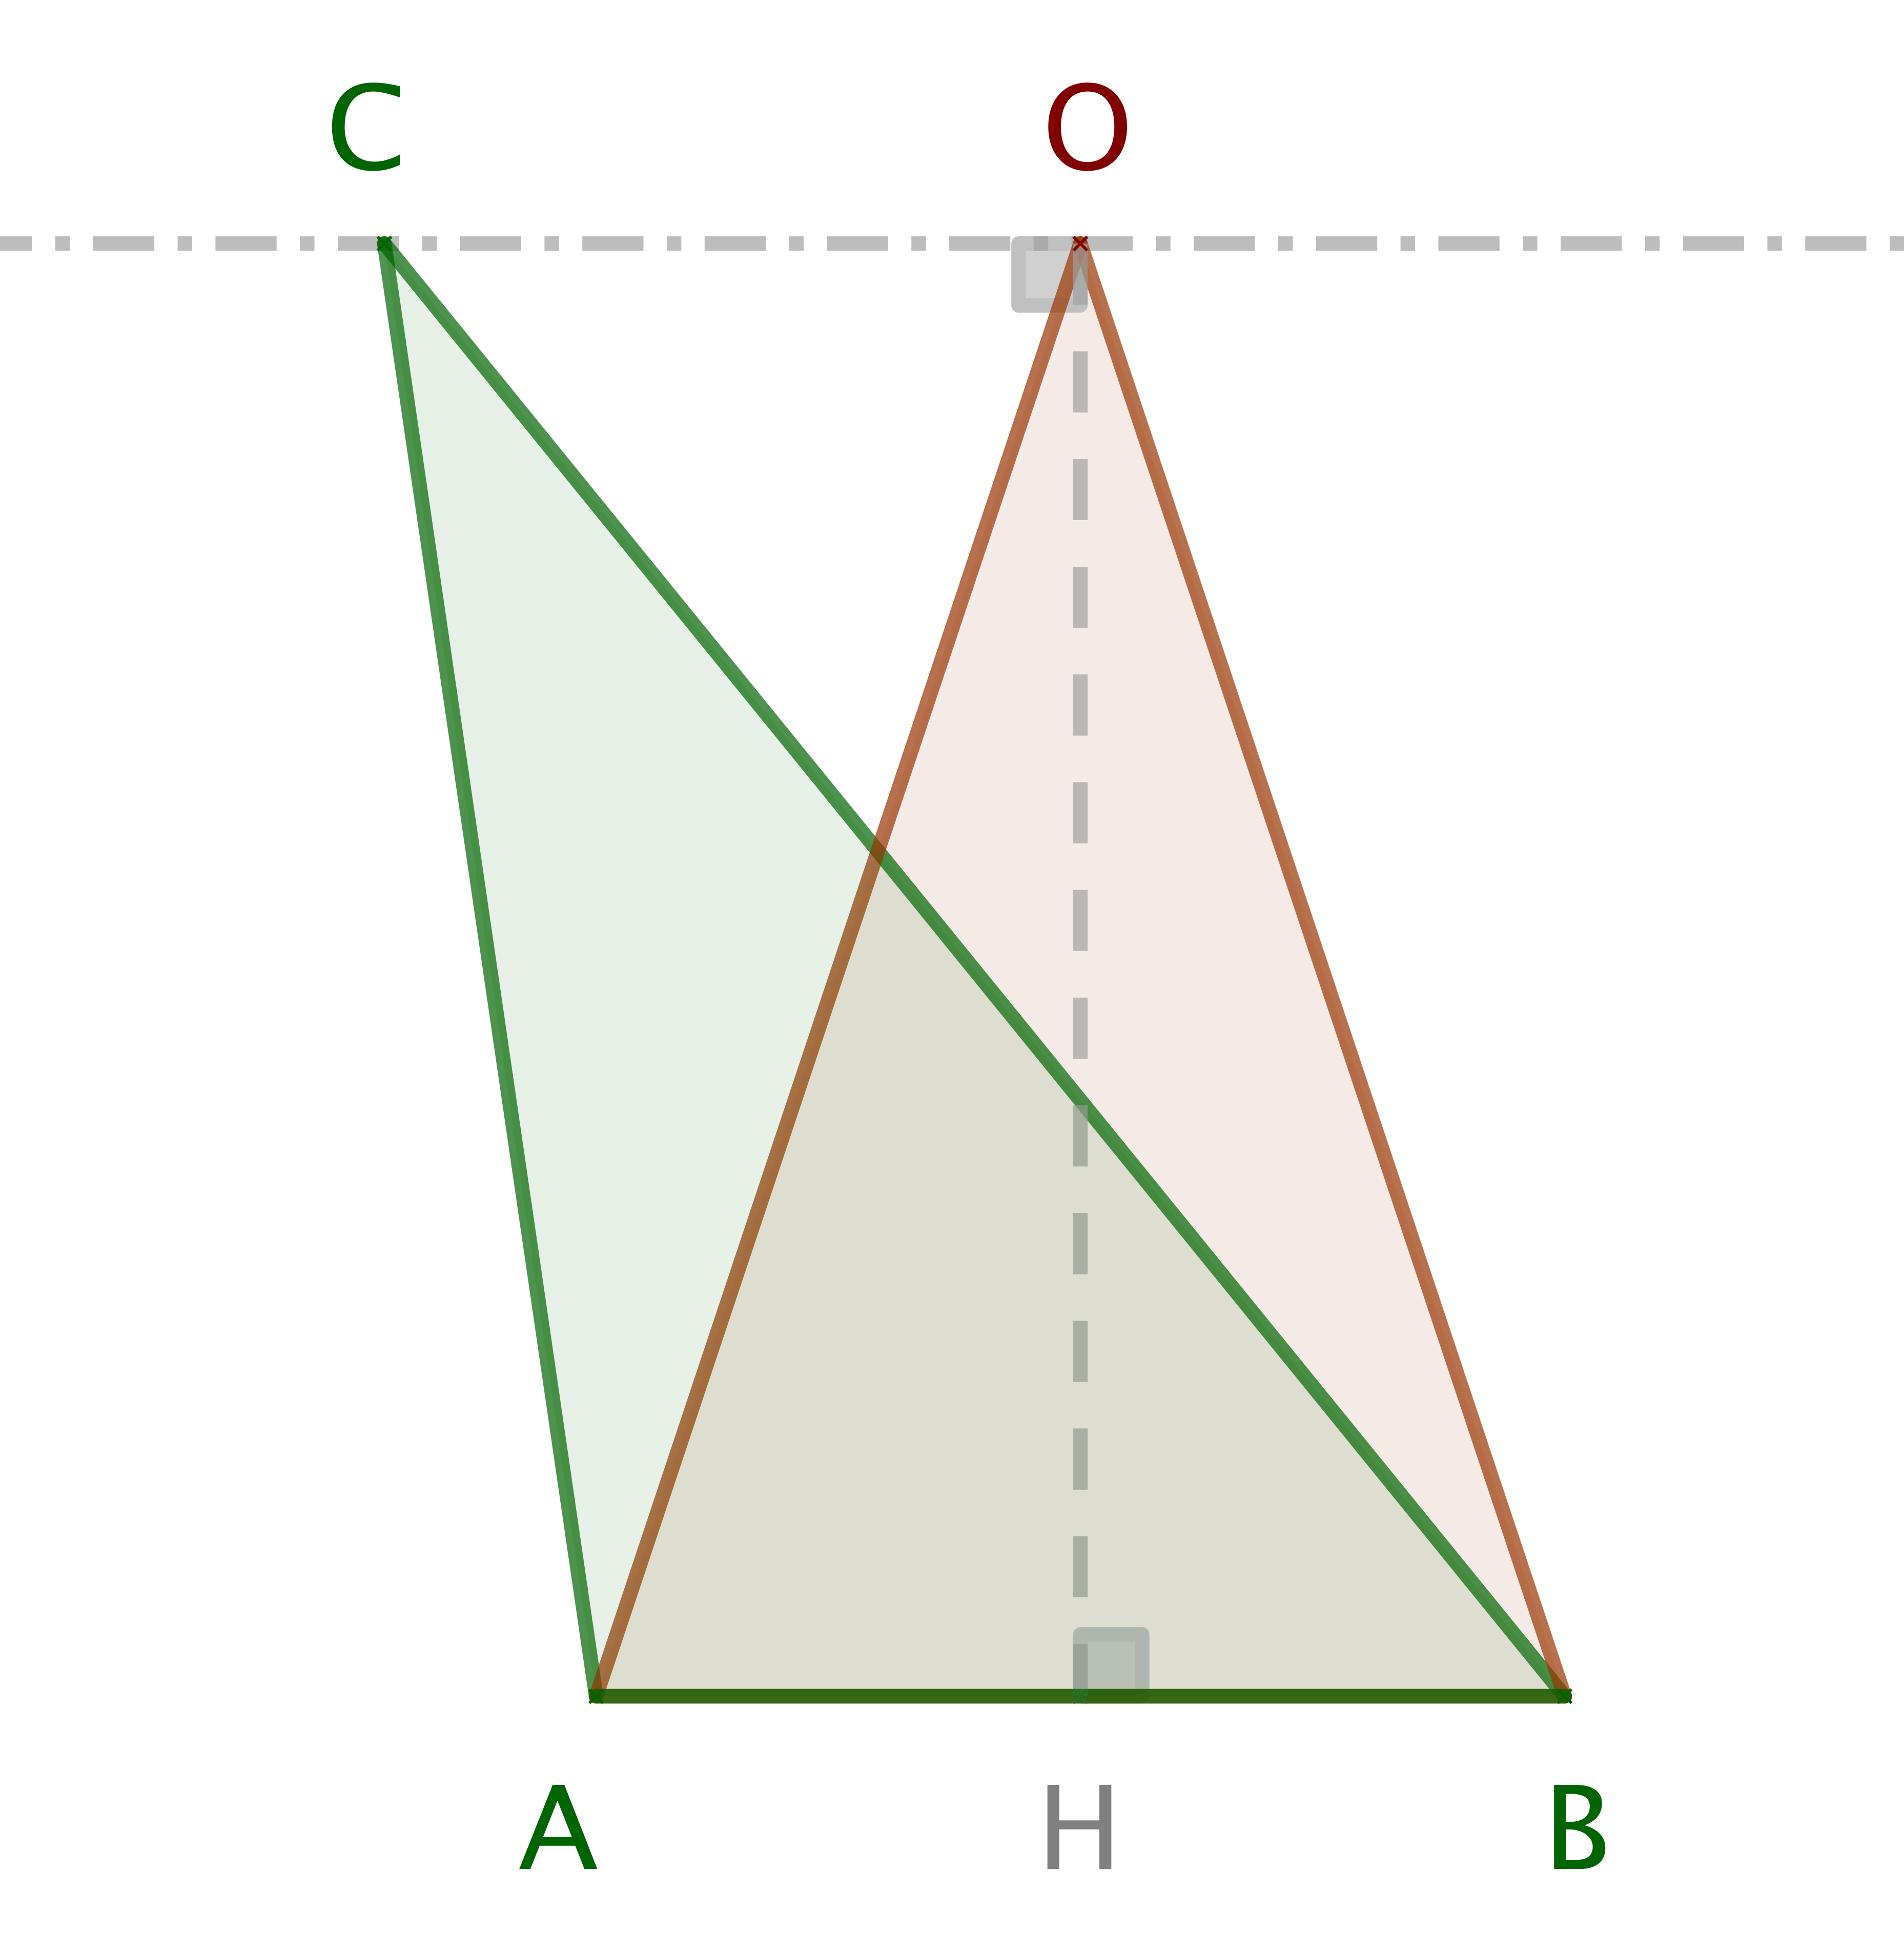
\includegraphics[scale=.4]{content/triangle-one-side-fixed/triangle.png}
	\end{center}

	
	Via une symétrie axiale, voir ci-dessous, il est aisé de noter que $\perim{ABC} \geq \perim{ABO}$, avec égalité uniquement si $ABC$ est isocèle en $C$.
	Plus précisément, en passant de $C$ à $O$, le périmètre diminue.
	
	\begin{center}
		\includegraphics[scale=.4]{content/triangle-one-side-fixed/proof.png}
	\end{center}
	
	Une dilatation \focus{verticale} de rapport $r = \frac{\perim{ABC}}{\perim{ABO}} \geq 1$ donne un triangle isocèle $ABO^{\,\prime}$ tel que 
	$\perim{ABO^{\,\prime}} = p$
	et 
	$\area{ABO^{\,\prime}} \geq \area{ABC}$, avec égalité uniquement si $ABC$ est isocèle en $C$. 
	Contrat rempli!%
	\footnote{
		Dans la section \ref{constrained-extrema} est expliqué comment employer la méthode des extrema liés. 
		Les arguments fournis à cet endroit s'adaptent facilement au cas des triangles de base fixée.
	}
\end{proof}


% ----------------------- %


\begin{remark}
	La recherche parmi les triangles avec un côté fixé de celui ayant un périmètre minimal pour une aire fixée est le problème dual de l'isopérimétrie pour ces triangles.
\end{remark}

%

%% ------------- %
%
%
\section{Les triangles sans contrainte}

\begin{fact} \label{iso-tri}
	Considérons tous les triangles de périmètre fixé $p$. Parmi tous ces triangles, un seul est d'aire maximale, c'est le triangle équilatéral de côté $c = \dfrac13 p$.
\end{fact}


\begin{proof}	
	Nous allons donner une démonstration constructive via une application itérative du fait \ref{tri-one-side-fixed} qui va donner à la limite le triangle équilatéral d'aire maximale, et ceci avec une vitesse de convergence exponentielle.%
	\footnote{
		Ceci ne va nécessiter que l'emploi de propriétés simples de l'ensemble des réels.
	}
	Partons donc d'un triangle $ABC$ quelconque, mais de périmètre $p$, le fait \ref{tri-one-side-fixed} nous donne successivement les triangles $ACD$, $ADE$ et $AEF$ isocèles en $D$, $E$ et $F$ respectivement, ayant tous pour périmètre $p$, et ceci avec des aires de plus en plus grandes.  
	Le dessin suivant amène à conjecturer qu'en poursuivant le procédé pour avoir ensuite un triangle $AFG$ isocèle en $G$...\,, nous aboutirons \focus{à la limite} à un triangle équilatéral.

	\begin{center}
		\includegraphics[scale=.4]{content/triangle-gene/proof.png}
	\end{center} 

	
	Le passage d'un triangle quelconque $ABC$ au triangle $ACD$ isocèle en $D$ nous amène à nous concentrer sur ce que donne notre procédé d'agrandissement d'aire à périmètre fixé pour des triangles isocèles. 
	Voici ce que nous pouvons affirmer en supposant $AC > AD$, comme dans notre exemple (nous allons voir que cette hypothèse est sans conséquence).
	%
	\begin{enumerate}
		\item Comme $AC + 2 AD = p$ et $AC > AD$, nous avons $AC > \frac13 p > AD$.
		À l'étape suivante, comme $AD + 2 AE = p$, nous obtenons $AD < \frac13 p < AE$.


		\item Pour $AEF$ isocèle en $F$, comme $AE + 2AF = p$, nous arrivons à  $AE > \frac13 p > AF$.
		
		
		\item \label{tri-equi-conv}
		Tentons de quantifier les écarts à la mesure pivot $p^{\,\prime} = \frac13 p$. 
		%
		\begin{itemize}
			\item Dans $ACD$, posant $AD = p^{\,\prime} - \epsilon_1$, nous avons $AC = p^{\,\prime} + 2 \epsilon_1$.

			\item Dans $ADE$, posant $AE = p^{\,\prime} + \epsilon_2$, nous avons $AD = p^{\,\prime} - 2 \epsilon_2$.

			\item Dans $AEF$, posant $AF = p^{\,\prime} - \epsilon_3$, nous avons $AE = p^{\,\prime} + 2 \epsilon_3$.

			\item Dans $AFG$, posant $AG = p^{\,\prime} + \epsilon_4$, nous avons $AF = p^{\,\prime} - 2 \epsilon_4$.

			\item Donc
			$\epsilon_2 = \frac12 \epsilon_1$,
			$\epsilon_3 = \frac12 \epsilon_2$
			et
			$\epsilon_4 = \frac12 \epsilon_3$.
		\end{itemize}
	\end{enumerate}


	\smallskip
	
	Voici les enseignements de ce qui précède en partant d'un triangle $ABC$ non équilatéral.
	%
	\begin{itemize}
		\item Si $AC = \frac13p$, dès la 1\iere\ itération, nous avons un triangle équilatéral d'aire plus grande.
		
		
		\item Si $AC \neq \frac13p$, notre procédé n'arrivera jamais en un nombre fini d'étapes à un triangle équilatéral.
		Dans ce cas, le point \ref{tri-equi-conv} ci-dessus nous donne une convergence exponentielle des longueurs des côtés vers $p^{\,\prime} = \frac13 p$, tout en ayant des aires des plus en plus grandes.
	\end{itemize}
	
	Dans tous les cas, l'aire d'un triangle non équilatéral de périmètre $p$ est strictement majorée par celle du triangle équilatéral de périmètre $p$. Et tout ceci a été obtenu via de la géométrie et de l'analyse élémentaires!
\end{proof}

%
%
%% ------------- %
%
%
%\section{Les quadrilatères}
%
%\begin{fact}
	Considérons tous les quadrilatères de périmètre fixé $p$. Parmi tous ces quadrilatères, celui d'aire maximale est le carré de côté $c = \num{.25} p$.
\end{fact}


\begin{proof}
	La figure suivante montre que pour tout quadrilatère $ABCD$ non convexe en $B$, et de périmètre $p$, il existe un quadrilatère convexe $AB^{\,\prime}CD$ de périmètre $p$, et tel que $\area{AB^{\,\prime}CD} \geq \area{ABCD}$.
	Notre recherche doit donc continuer dans l'ensemble des quadrilatères convexes de périmètre $p$.

	\begin{center}
		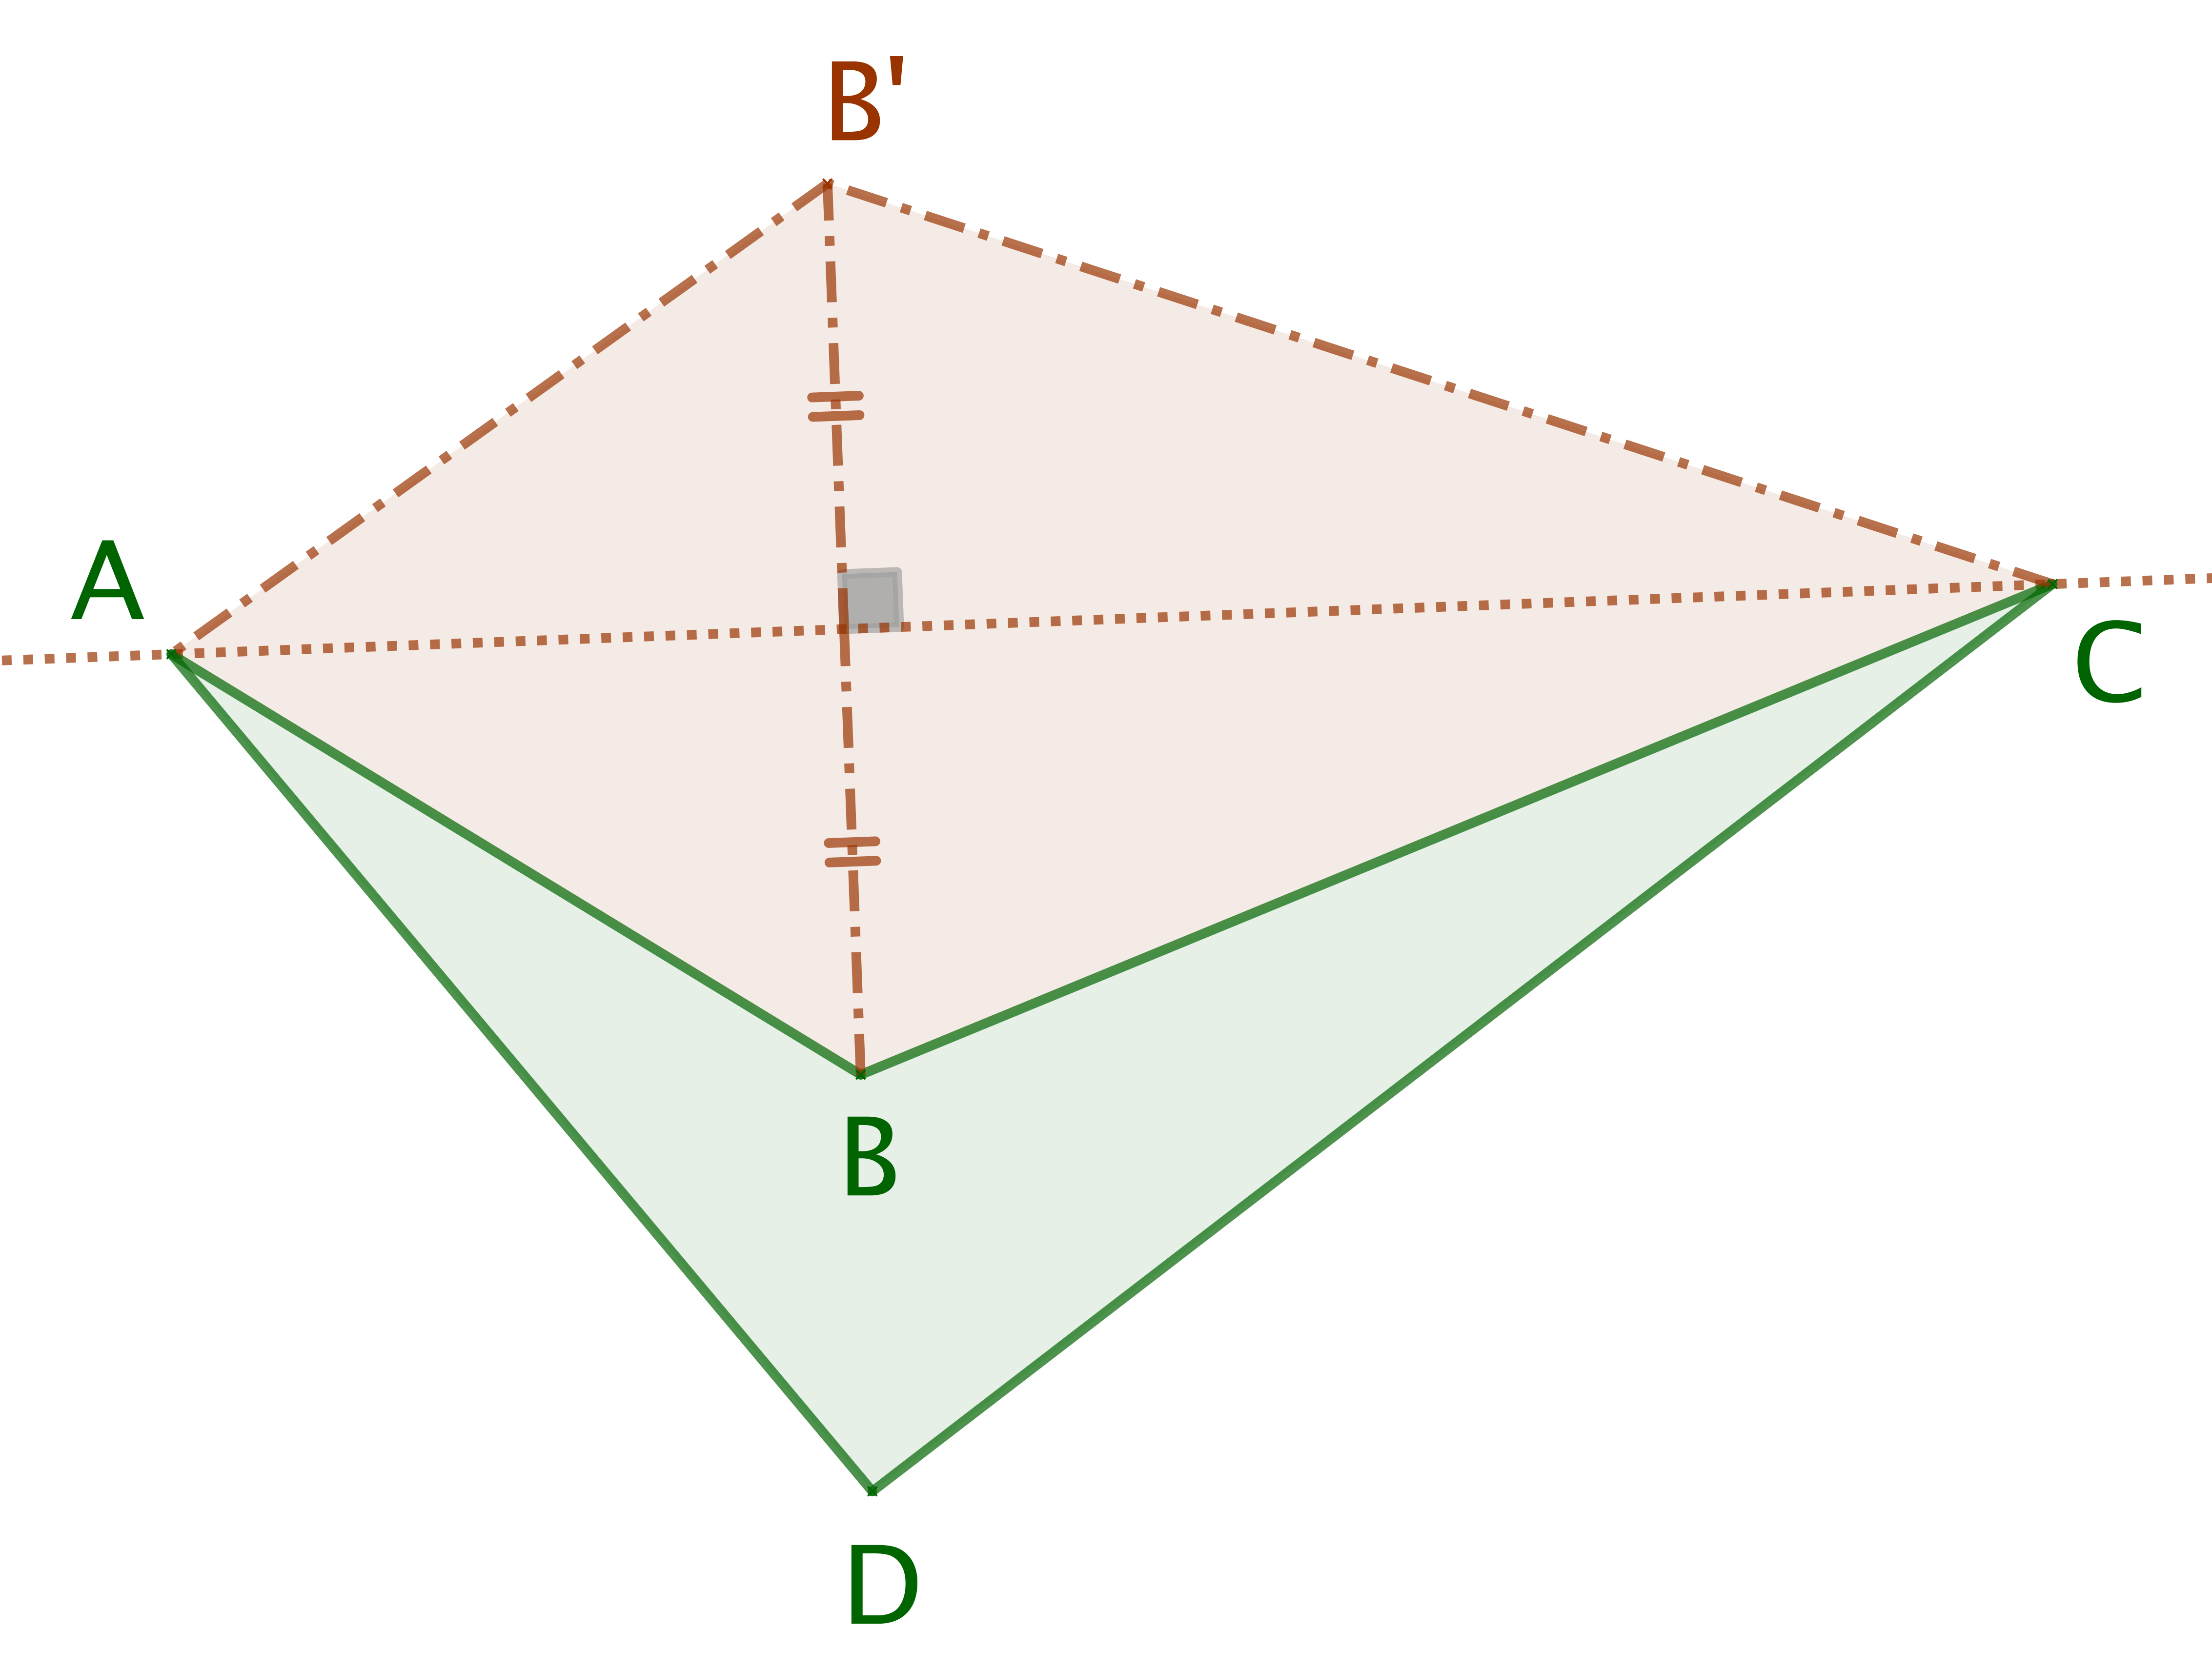
\includegraphics[scale=.4]{content/quadrilateral/quadrilateral-non-convex.png}
	\end{center}
	
	
	Comme dans la preuve du fait \ref{iso-tri-one-side-fixed}, à partir d'un quadrilatère convexe $ABCD$ de périmètre $p$, nous obtenons un quadrilatère convexe $AB^{\,\prime}CD$ de périmètre $p$,%
	\footnote{
		Noter que
		$\perim{AB^{\,\prime}CD} = \perim{AB^{\,\prime}C} + \perim{ACD} - 2 AC$.
	}
	et tel que $AB^{\,\prime} = B^{\,\prime}C$ et $\area{AB^{\,\prime}CD} \geq \area{ABCD}$ comme le montre la figure ci-après. 

	\begin{center}
		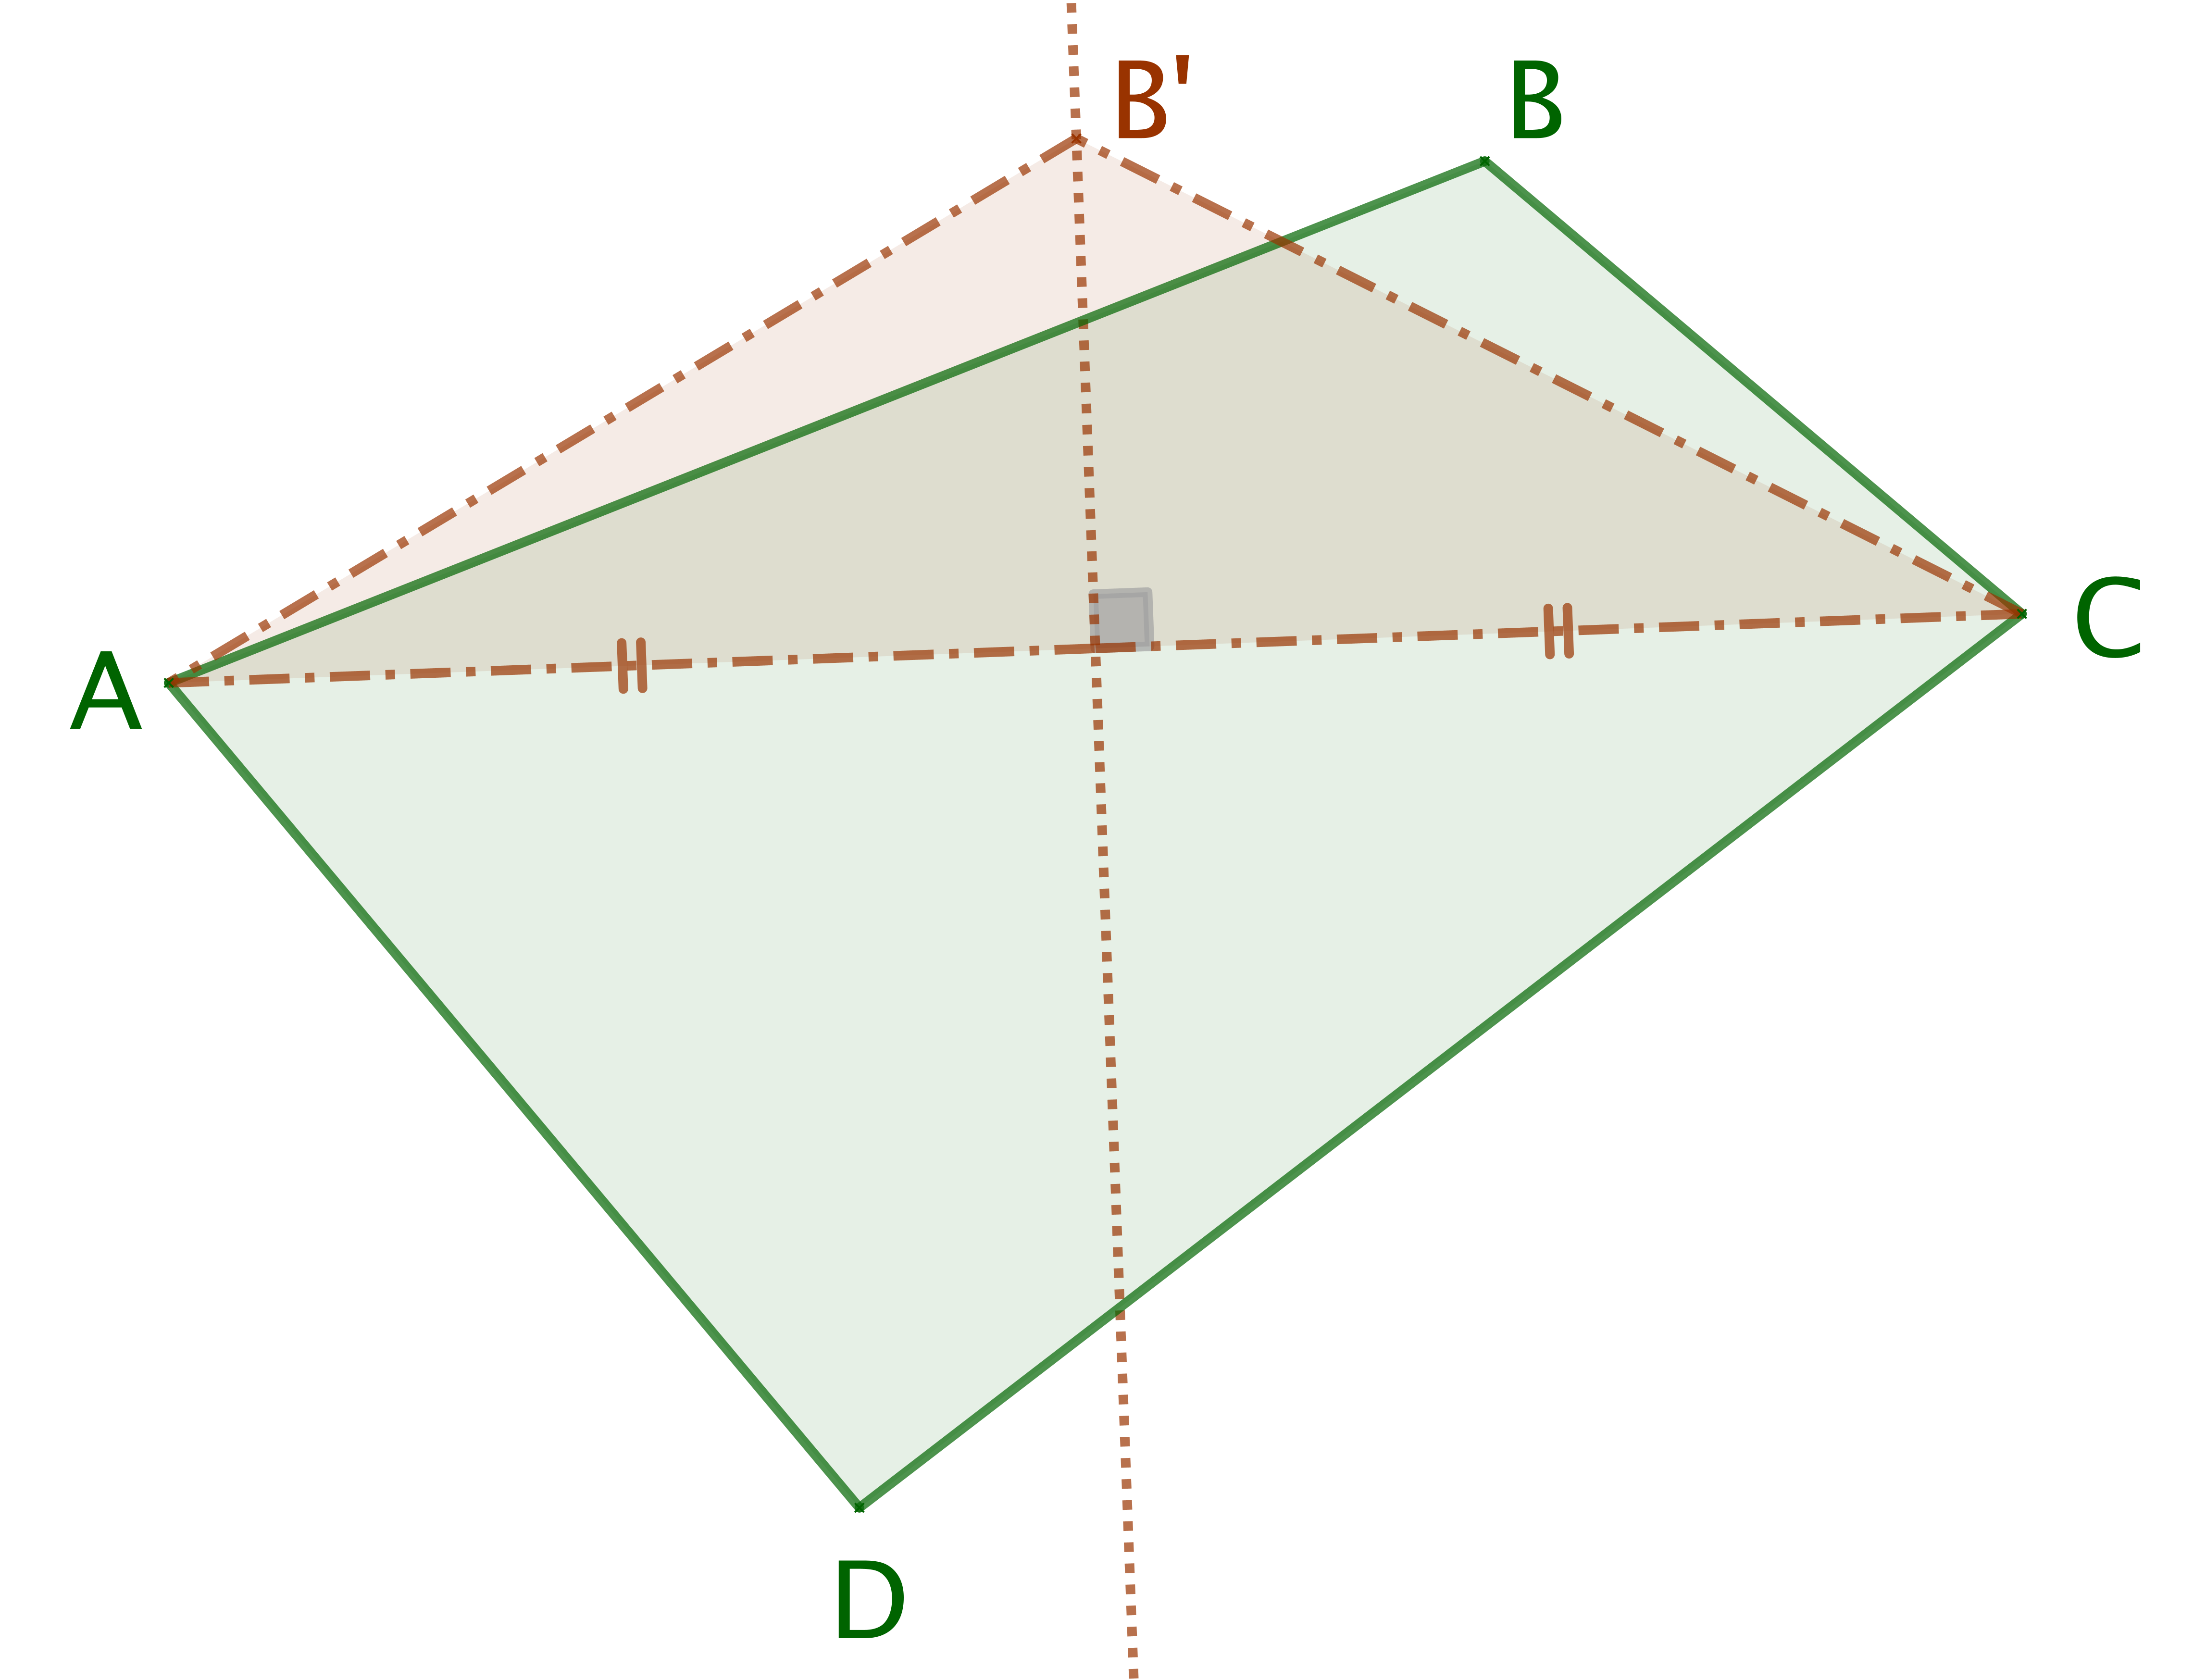
\includegraphics[scale=.4]{content/quadrilateral/quadrilateral-convex-gene.png}
	\end{center}
	
	
	La méthode précédente appliquée au sommet $D$ donne un cerf-volant $ABCD$ de périmètre $p$, et tel que $AB = BC$ et $AD = DC$, voir ci-dessous. 
	Cette même méthode avec les sommets $A$ et $C$ fournit un losange $A^{\,\prime}BC^{\,\prime}D$ de périmètre $p$, et tel que $\area{A^{\,\prime}BC^{\,\prime}D} \geq \area{ABCD}$.
	%
	En effet, nous avons
	$p = 2(AB + AD)$
	et
	$\perim{A^{\,\prime}BD} = \perim{ABD}$,
	donc
	$A^{\,\prime}B = A^{\,\prime}D = \num{.25} p$,
	et de même, nous obtenons
	$C^{\,\prime}B = C^{\,\prime}D = \num{.25} p$.

	\begin{center}
		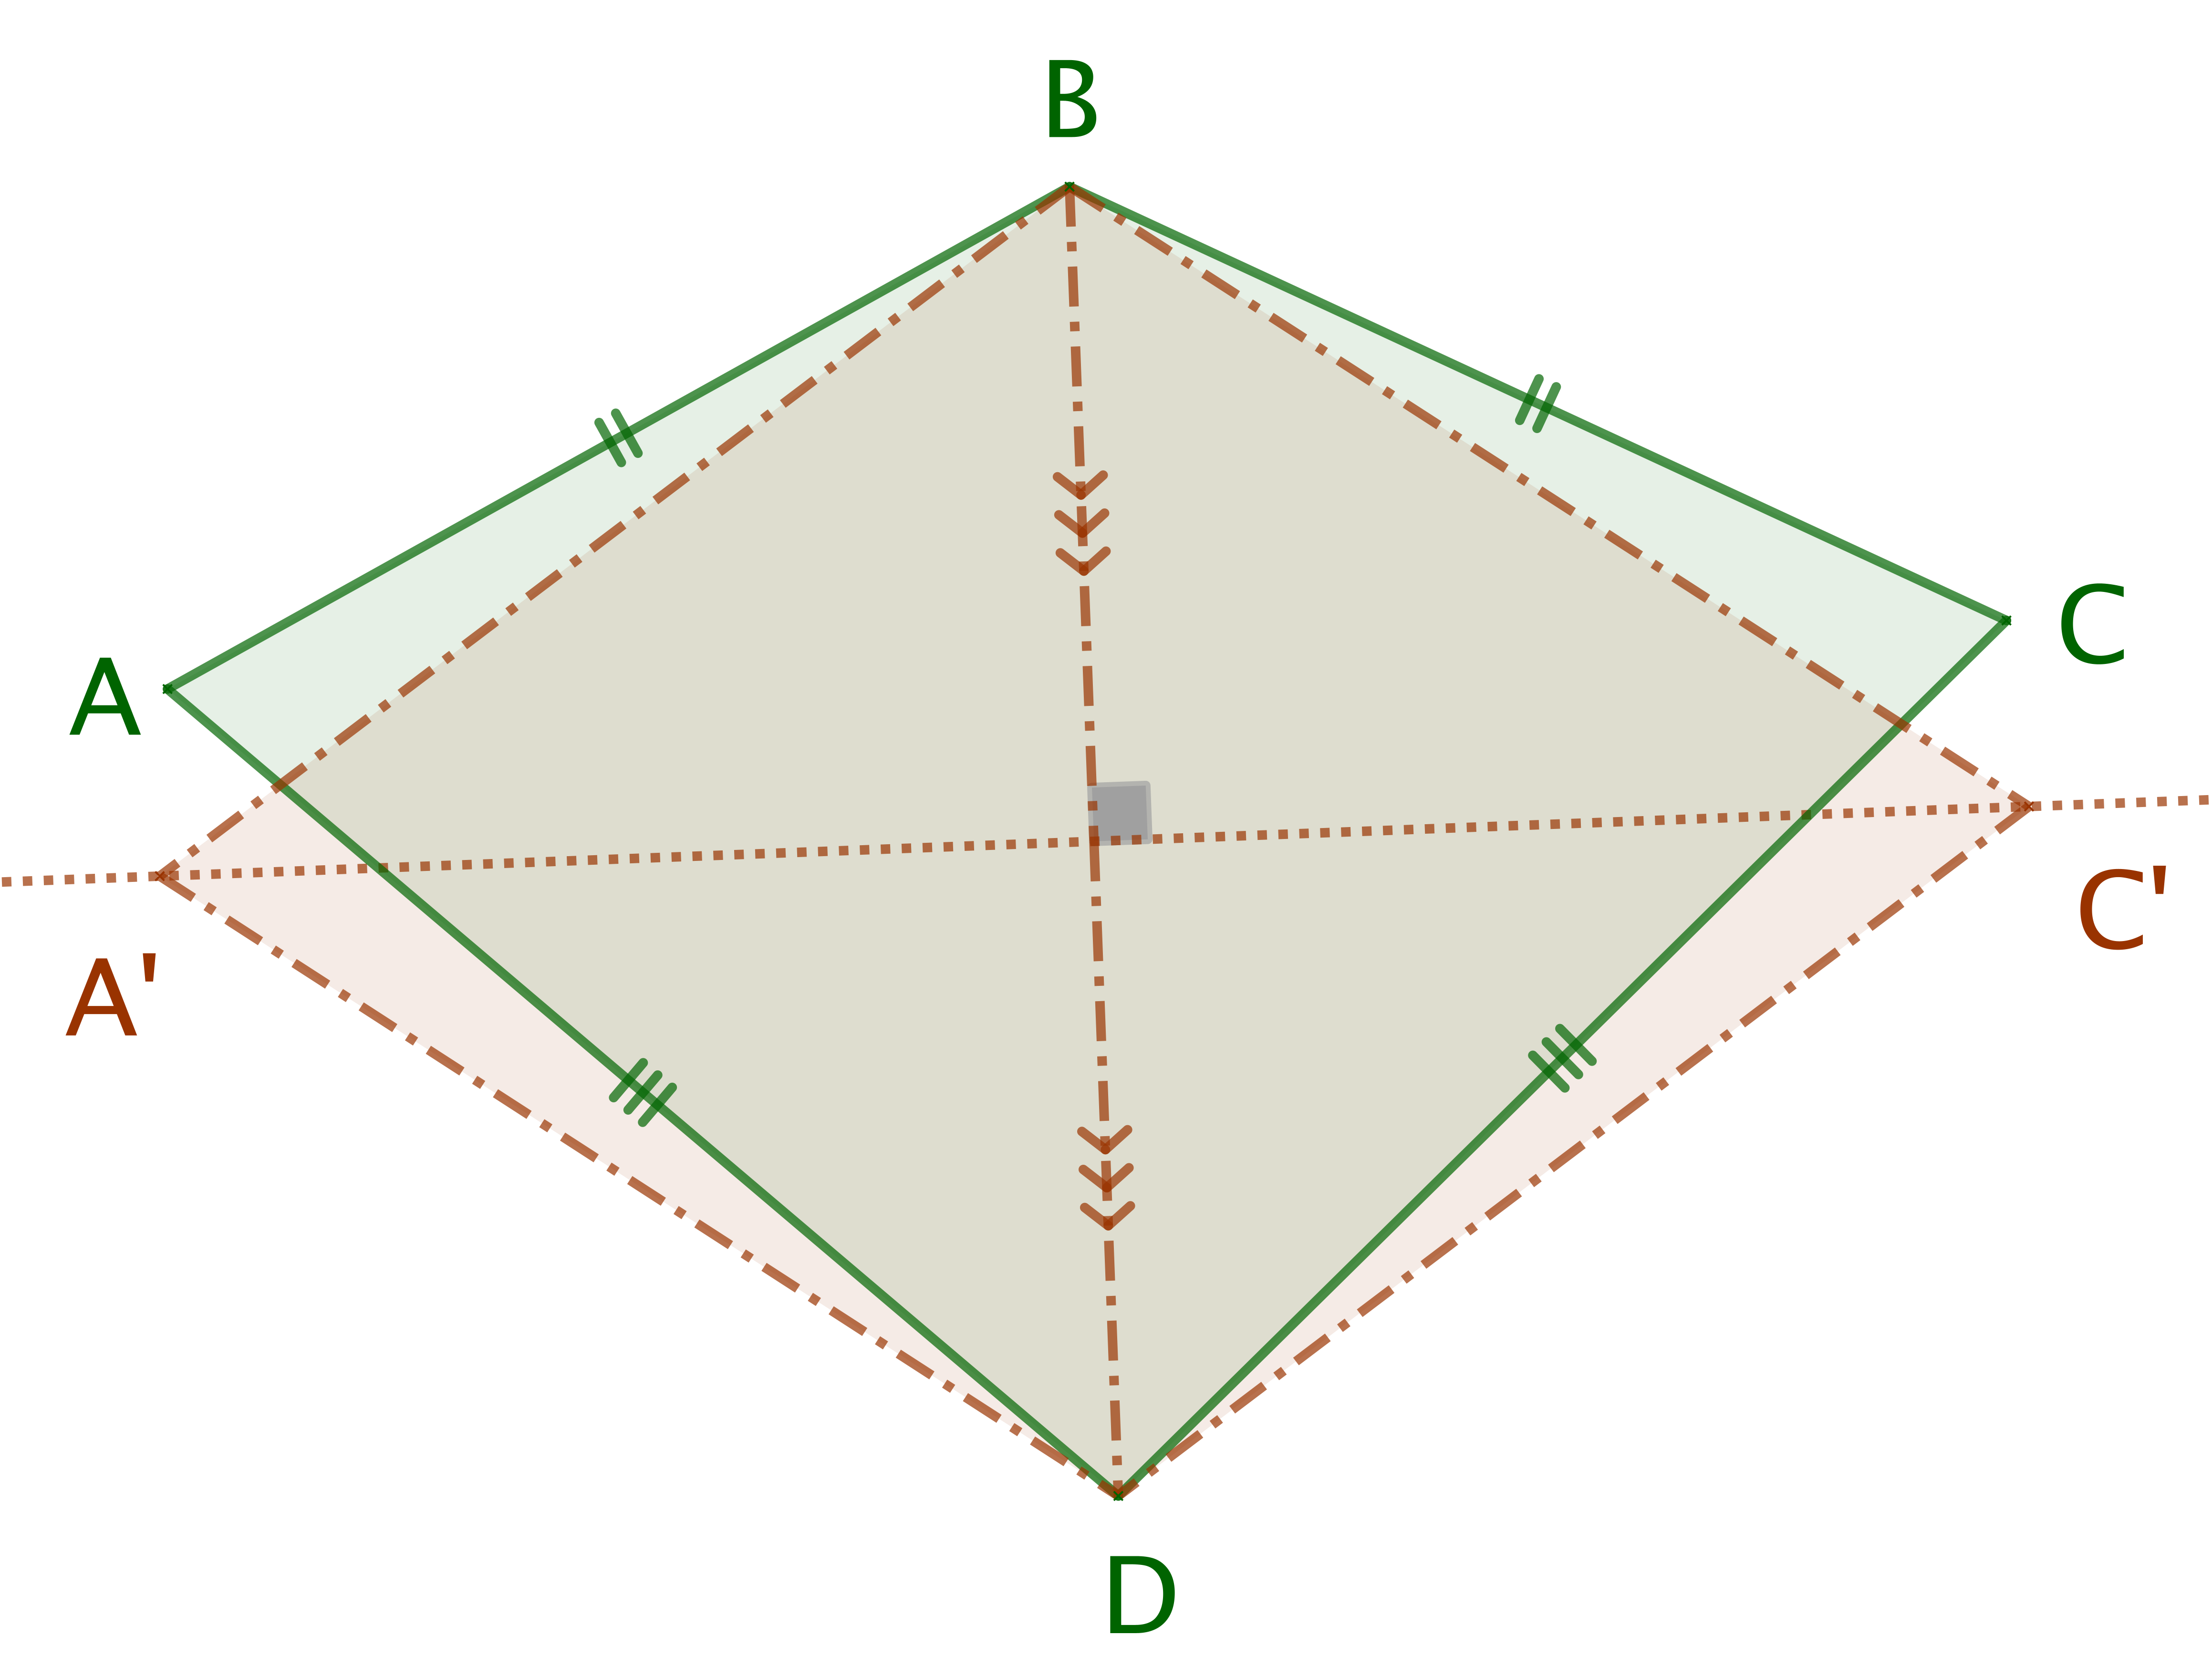
\includegraphics[scale=.4]{content/quadrilateral/quadrilateral-convex-isopaire.png}
	\end{center}
	
	
	Pour conclure, il suffit d'appliquer le fait \ref{iso-para}, puisque tout losange est un parallélogramme. Que la géométrie est belle!
\end{proof}



\end{document}
